\documentclass{homework}

\title{Homework 3}
\author{Kevin Evans}
\studentid{11571810}
\date{September 15, 2021}
\setclass{Math}{364}
\usepackage{amssymb}
\usepackage{mathtools}
\usepackage{graphicx}
\usepackage{amsthm}
\usepackage{amsmath}
\usepackage{slashed}
\usepackage{boldline}
\usepackage{physics}
\usepackage{tcolorbox}
\usepackage[inter-unit-product =\cdot]{siunitx}

\usepackage[makeroom]{cancel}
\usepackage{booktabs}
\usepackage{multirow}

\usepackage{times}
\usepackage{mhchem}

%\usepackage{calligra}
%\DeclareMathAlphabet{\mathcalligra}{T1}{calligra}{m}{n}
%\DeclareFontShape{T1}{calligra}{m}{n}{<->s*[2.2]callig15}{}
%\newcommand{\scriptr}{\mathcalligra{r}\,}
%\newcommand{\boldscriptr}{\pmb{\mathcalligra{r}}\,}
%\newcommand{\emf}{\mathcal{E}}
\newcommand{\st}{\mathrm{s.t.}}

\begin{document}
	\maketitle
	\begin{enumerate}
		\item Find the largest circle contained in the polygon
		\[ P=\left\{x\in\mathbb{R}^2\mid\:a_kx_1+b_kx_2\le c_k,\:k=1,2,\cdots,n; \text{with}~a_k^2+b_k^2=1\right\}. \]
		Suppose $(x_1, x_2) \in P$, then the signed-distance from $x$ to the line $a_k x_1 + b_k x_2 = c_k$ is $d_k(x) = \left(c_k - a_k x_1 - b_k x_2\right)$, where positive distances correspond to points in the corresponding halfspace and negative distances correspond to points outside the halfspace. 
		
		To find the largest circle, you must find the center point $x \in P$ that maximizes the signed-distance to the closest line defined by the polygon boundary.  This maximal distance is the radius of the largest possible circle. That is, the goal is $\max_x(\min_k d_k(x))$. Formulate this problem as a linear program.
		
		\textit{Solution.} \quad The decision variables are the location of the circle and its radius, \begin{align*}
			\text{Let } x & = \text{the location of the circle in $\mathbb{R}^2$} \\
				r & = \text{the radius of the circle}.
		\end{align*}
	
		The objective function is the radius of the circle that we're maximizing, $r$.
		
		The constraints are given by whether the points lay within the polygon or beyond it: for all $k$, $d_k \ge 0$ and ensuring that $x$ is within the polygon, $x \in P$ (I'm not sure if this constraint makes sense).
		
		\begin{tcolorbox}
			\vspace{-1em}
			\begin{align*}
				\max_{x \in \mathbb{R}^2, r \in \mathbb{R}} \quad & z=r \\
				\st \quad & d_k \ge 0 \qquad \text{for } k = 1, 2, \dots, n\\
					& x \in P?\\
				\text{where} \quad & P=\left\{x\in\mathbb{R}^2\mid\:a_kx_1+b_kx_2\le c_k,\:k=1,2,\cdots,n; \text{with}~a_k^2+b_k^2=1\right\} \\
				& d_k(x) = \left(c_k - a_k x_1 - b_k x_2\right)
			\end{align*}
		\end{tcolorbox}
		
		\pagebreak
		
		\item Consider a population model for bacteria in a closed environment given by $p(t) = A t^n e^{-t/\tau}$. The population at time $t$ is $p(t)$, where $A$, $n$, and $\tau$ are constants.
		
		\begin{enumerate}
			\item Plot or very carefully sketch $p(t)$ for $n=2, 3, 4$. Be sure and consider an appropriate range of values for $t\ge 0$ to illustrate plot features.
			
			\begin{center}
				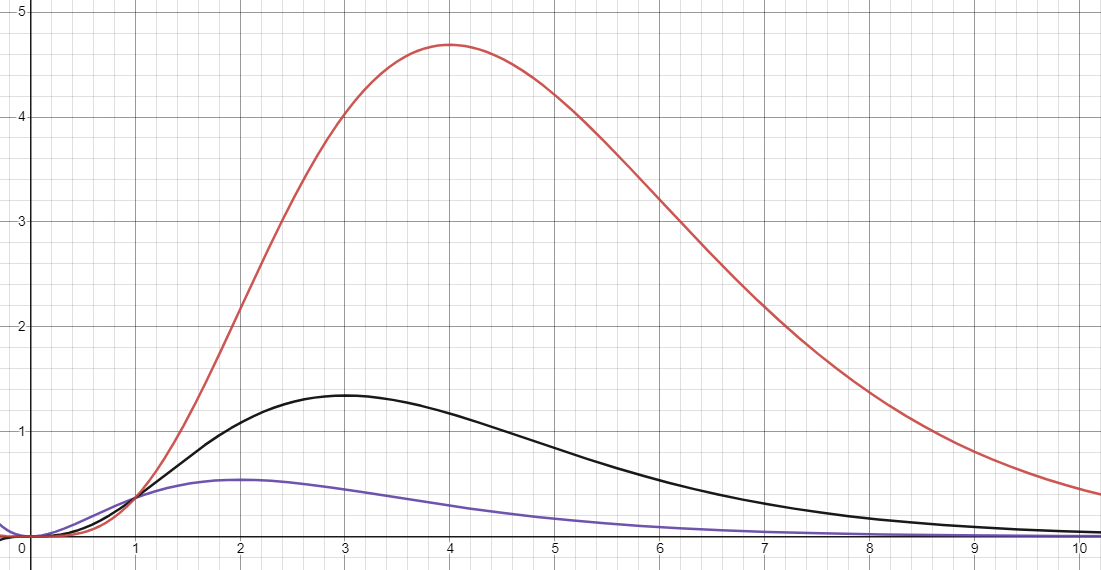
\includegraphics[width=\linewidth]{plot}
			\end{center}
			
		
			\item Using your plot features, explain why this model may be physically reasonable.  How do the constants  $A, n, \tau$ affect the population growth and decay?
			
			\vspace{1em} 
			\textit{Solution.} \quad It seems reasonable as it has an exponential curve that initially increases, slows down, then decreases as overpopulation (resource depletion) occurs. 
			
			\begin{itemize}
				\item $A$ affects the maximum population, i.e. the amplitude
				\item $n$ affects how quickly the maximum ramps up
				\item $\tau$ affects the how long the entire lifecycle takes
			\end{itemize}
			
			\item Consider a data set of time-population pairs, $\{(t_k, p_k)\}^N_{k=1}$. Formulate a linear program which can be used to solve the problem of fitting this data to the model using the method of least deviation.  The goal is to determine optimal coefficients $A, n, \tau$.  This cannot be done directly as outlined in class.  Instead, formulate the problem using the logarithm of the model function. 
			
			\vspace{1em}
	
			\textit{Solution.} \quad  The decision variables are the parameters of the fitting function $A$, $n$, and $\tau$.
			
			From the model function, we will take the log of it before applying the method of least deviation\footnote{Would it be possible to expand out the exponential instead of taking the log?}, \begin{align*}
				\ln(At^n e^{-t/\tau}) & = A \left(n \ln t - t/\tau\right)
				\intertext{The objective function is the sum of the absolute residuals,}
				z & = \sum_{k=1}^N \abs{ \hat{y}_k  - y_k} \\
					& = \sum_{k=1}^N \abs{ A \left(n \ln t_k - t_k/\tau\right) - \ln(p_k)}
			\end{align*}
			The constraints will come once we convert the absolute function to a LP. The complete linear program is 
			
			\begin{tcolorbox}
				\vspace{-1em}
				\begin{align*}
					\min_{\delta, A, n, \tau} \quad & \sum_{k=1}^N \delta_k \\
					\st \quad & \delta_k \ge A(n \ln t_k - t_k / \tau) - \ln(p_k) \\
						& \delta_k \ge -A(n \ln t_k - t_k / \tau) + \ln(p_k) \\
						& \delta \in \mathbb{R}^N \\
						& A, n, \tau \in \mathbb{R}
				\end{align*}
			\end{tcolorbox}
			
		\end{enumerate}
	\end{enumerate}
\end{document}